%%%%%%%%%%%%%%%%%%%%%%%%%%%
\newcommand{\documentName} { Examen 3ª evaluación }
\newcommand{\documentContent} { Estadística } 
\newcommand{\waterMark} { Modelo A } 
%%%%%%%%%%%%%%%%%%%%%%%%%%%

% Configuración del documento.
\newcommand{\schoolSubject} { Matemáticas 3º ESO - Recuperación}
\newcommand{\school} { IES La Serna }
\newcommand{\academicPeriod} { Curso 2020/2021 }


\newcommand{\autor} { Andrés Giménez Muñoz }
\newcommand{\emailAuthor} { agimenezmunoz@ieslaserna.com }
\newcommand{\autorSing}{ Profesores: Andrés } 
\renewcommand{\schoolSubject} { Examen Matemáticas 2º ESO  }
\renewcommand{\school} { IES José de Churriguera  }
\renewcommand{\academicPeriod} { Curso 2022/2023 }

\renewcommand{\autor} { Andrés Giménez Muñoz }
\renewcommand{\emailAuthor} { andresprofemates@outlook.es }
\renewcommand{\autorSing}{ Profesor: Andrés } 

%%%%%%%%%%%%%%%%%%%%%%%%%%%
% Exam configuration
%\pointsdroppedatright   %% No mostrar la puntuación
\pointsinrightmargin % Para poner las puntuaciones a la derecha. Se puede cambiar. Si se comenta, sale a la izquierda.
\extrawidth{-1.5cm} %Un poquito más de margen por si ponemos textos largos.
\marginpointname{ \emph{\points}}

%% Si se comenta no aparecerán los espacios de la solución.
%\nocancelspace

%% Esto es de la clase exam. Si dejamos sin comentar \printanswers, se mostraran las soluciones. 
%% Si la comentamos y dejamos sin comentar \noprintanswers, pues no se muestran las soluciones.
%\printanswers
%\noprintanswers

%%%%%%%%%%%%%%%%%%%%%%%%%%%

% \usepackage{tikz}
% \usetikzlibrary{arrows}

\begin{document}

	\StudentData
	\GradeTableHeader

    \justifying

	\begin{questions}
		\setcounter{question}{0}

		\question[3]
        En un club deportivo juvenil admiten socios con edades entre 12 y 18 años. La distribución de las edades es:
		\begin{table}[h!]
			\centering
			\begin{tabular}{|c|c|c|c|c|c|c|c|}
			\hline
			\cellcolor[gray]{0.8}Edad & 12 & 13 & 14 & 15 & 16 & 17 & 18 \\
			\hline
			\cellcolor[gray]{0.8}$f_i$ & 4 & 6 & 12 & 16 & 14 & 8 & 4 \\
			\hline
			\end{tabular}
		\end{table} 
        \\
        \begin{parts}
            \part
            Calcula las frecuencias relativas $(h_i)$ de la distribución.
            \part 
            % Moda = 15
            % Media = 15,09
            % Mediana = 15
		    Calcula la moda, la media aritmética y la mediana.
        \end{parts}
		\vspace{\stretch{1}}

        \newpage
        \question[2]
        En una fábrica de bombillas se estudia la vida de un tipo de bombilla. Se ha tomado una muestra de 200 lámparas con los siguientes resultados:
            \begin{table}[h!]
                \centering
                \begin{tabular}{|c|c|c|c|c|c|c|c|}
                \hline
                \cellcolor[gray]{0.8}Vida en horas & [100,300) & [300, 500) & [500, 700) & [700, 900) & [900, 1100] \\
                \hline
                \cellcolor[gray]{0.8}Nº bombillas & 10 & 65 & 75 & 35 & 15 \\
                \hline
                \end{tabular}
            \end{table} 

            Dibuja el histograma de la muestra: \\
            \begin{figure}[h]
                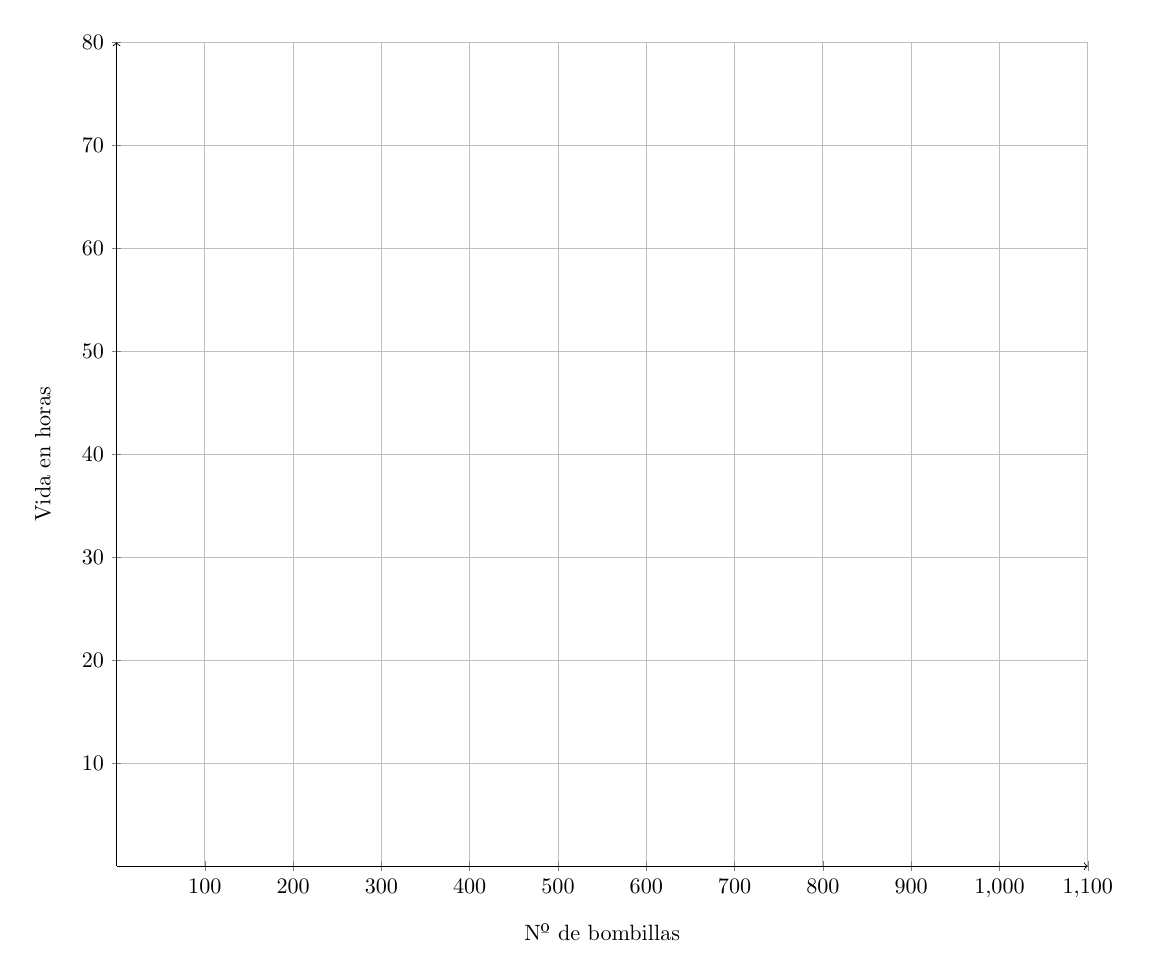
\begin{tikzpicture}[scale=0.8]
                    \begin{axis}[
                        axis lines=middle,
                        axis line style={->},
                        x label style={at={(axis description cs:0.5,-0.06)},anchor=north},
                        y label style={at={(axis description cs:-0.06,.5)},rotate=90,anchor=south},
                        xlabel={Nº de bombillas},ylabel={Vida en horas},
                        grid, width=17cm, xmax=1100,ymax=80,xmin=0,ymin=0,
                        %axis lines=middle
                        ]
                    \end{axis}
                \end{tikzpicture}
            \end{figure}

        \newpage
        \question[5]
        Para estudiar la repoblación forestal en una montaña se han medido las alturas de 40 árboles en cada vertiente: \\
        Vertiente norte:
        \begin{table}[h!]
			\centering
			\begin{tabular}{|c|c|c|c|c|c|c|c|}
			\hline
			\cellcolor[gray]{0.8}Altura (m) & [2,4) & [4,6) & [6,8) & [8,10) & [10, 12]\\
			\hline
			\cellcolor[gray]{0.8}Nº árboles & 7 & 9 & 10 & 8 & 6 \\
			\hline
			\end{tabular}
		\end{table} 
        \\
        Vertiente sur:
        \begin{table}[h!]
			\centering
			\begin{tabular}{|c|c|c|c|c|c|c|c|}
			\hline
			\cellcolor[gray]{0.8}Altura (m) & [2,4) & [4,6) & [6,8) & [8,10] \\
			\hline
			\cellcolor[gray]{0.8}Nº árboles & 4 & 10 & 18 & 8 \\
			\hline
			\end{tabular}
		\end{table} 
        \\
        \begin{parts}
            \part 
                % media = 6.5
                Si la media de la vertiente norte es $\bar{x}=6,85m$, calcula la media de la vertiente sur.
                \begin{equation*}
                    \bar{x}=\frac{\sum{x_i f_i}}{N} = \sum{x_i h_i}
                \end{equation*}
                \vspace{\stretch{1}}
            \part 
                % varianza = 3,15 y Desviación típica = 1,77.
                La varianza y la desviación típica de la vertiente norte son ${s^2=8,67m^2}$ y ${s=2,95m}$, calcula la varianza y desviación típica de la vertiente sur.
                \begin{equation*}
                    s^2=\frac{\sum{({x_i - \bar{x}})^2} f_i}{N} = \frac{\sum{{x_i}^2 f_i}}{N} - \bar{x}^2 = \sum{{x_i}^2 h_i} - \bar{x}^2
                \end{equation*}

                \begin{equation*}
                    s=\sqrt{\frac{\sum{({x_i - \bar{x}})^2} f_i}{N}} = \sqrt{\frac{\sum{{x_i}^2 f_i}}{N} - \bar{x}^2} = \sqrt{\sum{{x_i}^2 h_i} - \bar{x}^2}
                \end{equation*}
                \vspace{\stretch{2}}
                \newpage
            \part
                % CV = 0,27
                Si el coeficiente de variación para la vertiente norte es ${CV = 0,95}$, halla el coeficiente de variación de ambas distribuciones.
                \begin{equation*}
                    CV = \frac{s}{\bar{x}}
                \end{equation*}
                \vspace{\stretch{1}}
            \part
                ¿En cuál es la más representativa la media?
                \vspace{\stretch{1}}
            \part
                ¿En qué vertiente se prudce un crecimiento más uniforme?
                \vspace{\stretch{1}}
        \end{parts}
	\end{questions}
\end{document}